\subsection{The cell}
\label{sec:cell}
Cells are the fundamental units of every living being, which can be made up of one cell (unicellular) or more (multicellular).
Indipendently on how big and complex an organism could be, each cell always maintains its individuality and its independence, but maintaining common structural proprieties.

The internal volume is defined by the \textit{cytoplasm}, which is a liquid solution where several insoluble particles stands, such as enzimes, \textit{RNA} and metabolites.
Moreover, it is possible to distinguish multiple organelles, such as \textit{ribosomes}, the \textit{endoplasmic reticulum}, the \textit{golgi comples},\textit{lisosomes} and the \textit{nucleus} (figure \ref{fig:cell}).
In particular, this last one has a the role of contain the genome, represented by the \textit{DNA}.

\begin{figure}[h]
\centering
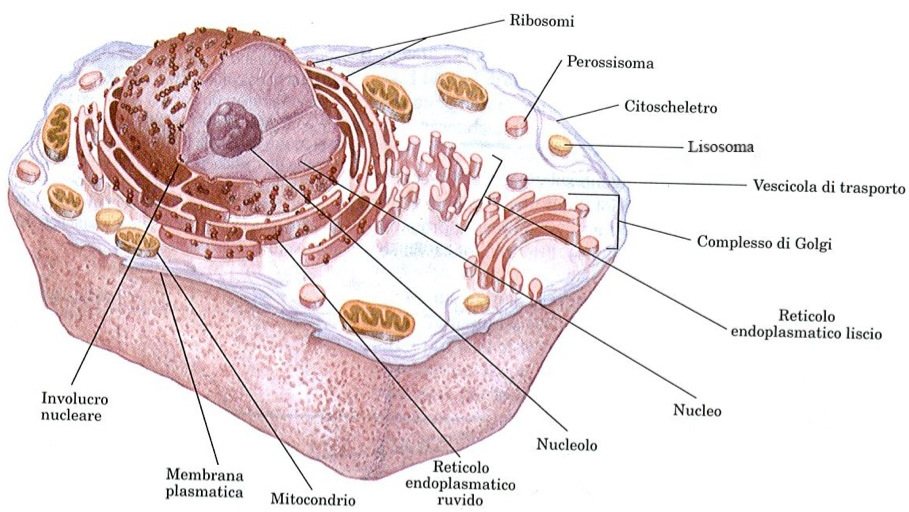
\includegraphics[width=10cm, keepaspectratio]{img/intro/cell.png}
\caption[The Cell]{Schematic representation of a cell.}
\label{fig:cell}
\end{figure}

\subsection{The DNA}
\label{sec:genica}
The \textit{DNA} was been isolated for the first time by the German doctor Friederick Miescher in 1869, while in the same decade the English biologist Charles Darwin was publishing \textit{On the Origin of the Species} and the  Augustinian friar scientist was communicating his results on the pees to the Brunn Natural History Society.

Because the substance isolated by Miescher was white, lightly acid and present only into the cells nuclei, it was been termed \textit{Nucleic Acid}.
Name modified afterwards in \gls{dna}, to distinguish is from the another one, very similar, the \gls{rna}.

These two molecules are constituted by \textit{nucleotides}, constituted by a nitrogen base, deoxyribose sugar and a phosphate group.
We distinguish two nitrogen bases, purines and pyrimidines.
Inside the \gls{dna}, we have two \textit{pyrimidines}, \textit{adenine (A)} and \textit{guanine (G)}, and two \textit{pyrimidines}, the \textit{Cytosine (C)} and the \textit{Thimine (T)}  .
Inside \gls{rna} \textit{Thymine} is substituted by the \textit{Uracil (U)}.

\begin{figure}[h]
\centering
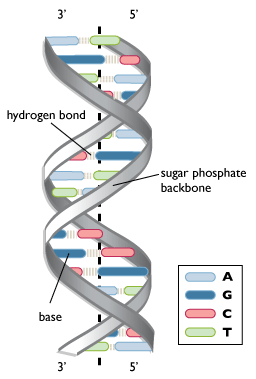
\includegraphics[width=5cm, keepaspectratio]{img/intro/dna1.png}
\caption[the \gls{dna}]{Schematic representation of double-stranded filament structure of \gls{dna}. The legend report the four nitrogen bases, Adenine, Guanine, Cytosine and Thymine.}
\label{fig:dna}
\end{figure}

\gls{dna} structure (figure \ref{fig:dna}) was discovered, in the 50's, by the American scientist James Watson, the French physicist Francis Crick and the English chemist-physicist Rosalind Franklyn.
According to their model the \gls{dna} is a double-stranded filament, where Adenines can pair only with Thymines and Guanines only with Cytosines.
The four bases constitute the alphabet for the genetic message.

\gls{dna} is folded on itself (\textit{\gls{dna} packaging}, thanks to specific "beads" called \textit{nucleosomes}, which themselves consist of eight proteins with tails, called \textit{histones}, that have the \gls{dna} wrapped on them.
This mechanism enables to store around 2 meters of chromatin inside a nucleus of a 2-10 micron diameter, when referring to Human specie.

Moreover, the \gls{dna} contains the \textit{genes}, particular sections containing relevant information for building proteins and other fundamental molecules for the cellular behavior regulation.
Each gene is localized on a precise position of a \textit{Chromosome}, which are in different number for each specie.
Each chromosome is constituted by \gls{dna} within thousands genes.

\begin{figure}[h]
\centering
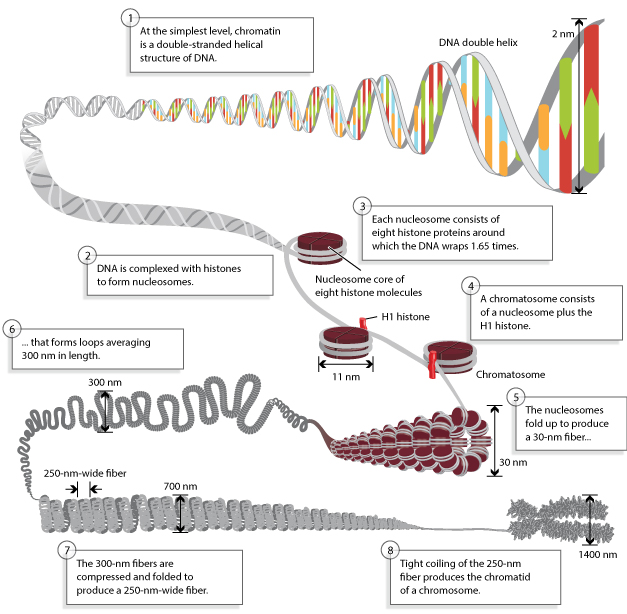
\includegraphics[width=8cm, keepaspectratio]{img/intro/dna2.jpg}
\caption[Chromosomes and \gls{dna}]{Representation of the relation between \gls{dna} and Chromosomes.
Inside the cell nucleus there are pairs of chromosome, constituted by chromatin, which fundamental unit is constituted by nucleosomes, on which the \gls{dna} is wrapped around, containing the genetic information in gene form. (image adapted from \cite{Annunziato2008})}
\label{fig:dnachromosome}
\end{figure}

Figure \ref{fig:dnachromosome} better helps  to understand the relationship between chromosomes, chromatin, nucleosomes and genes.

It is important to underlying that since some decades ago the Central Dogma of Molecular Biology was founded on the transcription - translation principle, where \gls{dna} was transcribed in \gls{rna}, which subsequently it would have been translated into protein.

Nowadays, we know that the gene transcription is regulated by several mechanisms, and moreover, the translation is not the only process fated for \gls{rna}.

Indeed, for a transcription of a gene, there are some requisites to be respected, such as the accessible of that specific part of the chromatin, or the binding of specific proteins enabling the accession to the gene region, or the histone modification processes, such as \textit{Acetylation}, \textit{Methylation}, \textit{Phosphorylation}, and others, which modifies the state of specific histones, and influencing gene expression regulation. 
  
\begin{figure}[h]
\centering
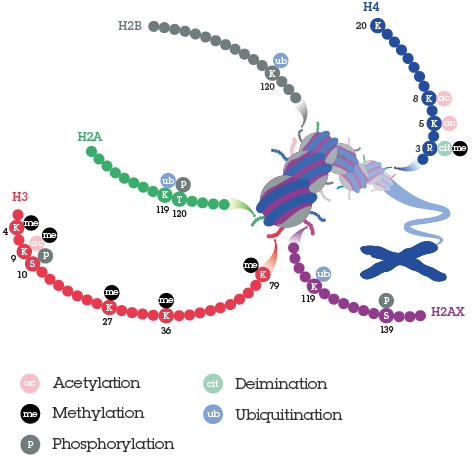
\includegraphics[width=8cm, keepaspectratio]{img/intro/hm.png}
\caption[Histon modification]{Representation of some processes involved in histone modification, influencing gene expression regulation.}
\label{fig:histmod}
\end{figure}
